\subsection{Results}
\label{cic:sec:Results-all}
Our analysis of survey and interview data focuses on how users navigate the spectrum between proxy-based and physical device control in everyday smart home use. We structure our findings around three core themes: (1) user strategies for navigating this spectrum (RQ1), (2) the tradeoffs they perceive when doing so (RQ1a),
(3) how navigation strategies, perspectives, and trust shift when users encounter device errors or failures (RQ2, RQ2a), and (4) how users commonly struggle to realize their goals across the control spectrum (RQ2b).

\subsubsection{Control spectrum navigation strategies (RQ1)}
\label{cic:subsec:controlspectrum}

\begin{figure}[ht]
    \centering
    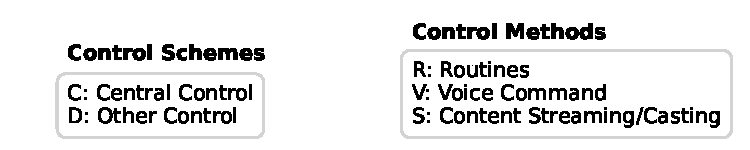
\includegraphics[width=0.667\textwidth]{ControlInContext/figures/control_schemes_legend_split.pdf}
    \vfill
    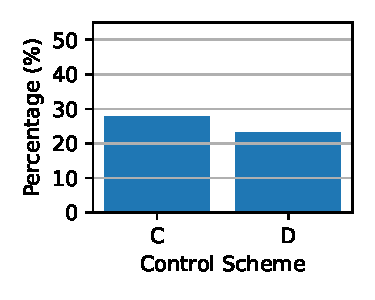
\includegraphics[width=0.3\textwidth]{ControlInContext/figures/control_schemes_popularity.pdf}
    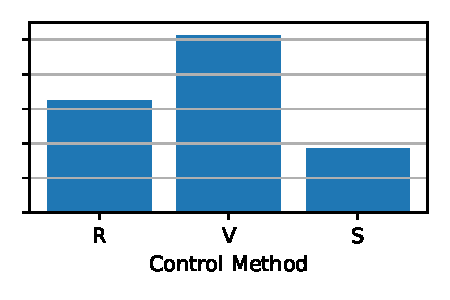
\includegraphics[width=0.36\textwidth]{ControlInContext/figures/control_methods_popularity.pdf}
    \caption{Percentage of participants using each control scheme/method.}
    \medskip
    \label{cic:fig:control-scheme-popularity}
\end{figure}

\begin{figure}[ht] %{0.5\textwidth}
    \centering
    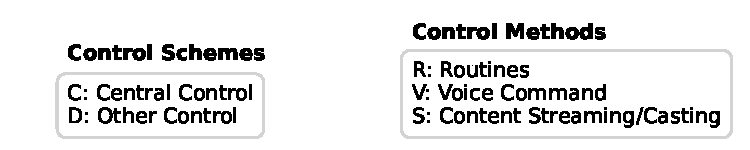
\includegraphics[width=0.667\linewidth]{ControlInContext/figures/control_schemes_legend_split.pdf}
    \par
    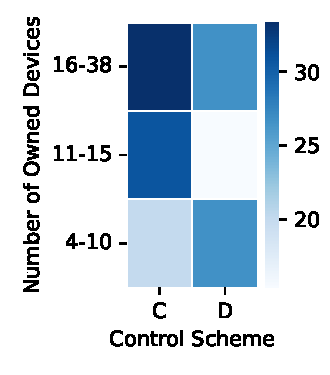
\includegraphics[width=0.268\linewidth]{ControlInContext/figures/control_schemes_vs_dev_no_bins.pdf}
    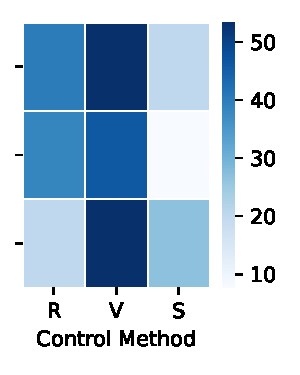
\includegraphics[width=0.24\linewidth]{ControlInContext/figures/control_methods_vs_dev_no_bins.pdf}
    \caption{Percentage of survey participants using central or other control schemes and several control methods vs. number of owned devices. Each cell's color shows the percentage of participants falling into it who choose the respective control scheme or method. The percentages for the different options of control schemes and methods do not add up to 100\% since the participants could provide multiple answers.}
    % \Description{Heatmaps showing percentages of participants using different control schemes and methods by number of owned devices.
    % 
    % The left heatmap compares control schemes: Central Control (C) and Other Control (D). Each row corresponds to a range of owned devices: 4-10, 11-15, and 16-38. Darker shades represent higher percentages. The highest usage of Central Control occurs in the 16-38 device group, followed by the 11-15 group. Other Control is most used by participants with either 4-10 or 16-38 devices, with lower use in the 11-15 range.
    % 
    % The right heatmap compares control methods: Routines (R), Voice Command (V), and Content Streaming/Casting (S), using the same device count bins. Voice Command consistently shows the darkest shading across all device ranges, especially in the lower two bins. Routines show moderate use across device ranges, while Content Streaming is most used in the lowest and highest device bins.
    
    %     Legend boxes at the top explain abbreviations for schemes and methods.
    % }

    \label{cic:fig:control-scheme-popularity-vs-dev-no}
\end{figure}

\begin{figure}[ht]
    \centering
    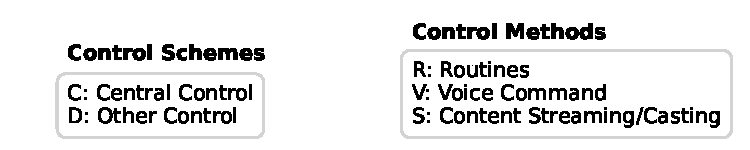
\includegraphics[width=0.667\linewidth]{ControlInContext/figures/control_schemes_legend_split.pdf}
    \par
    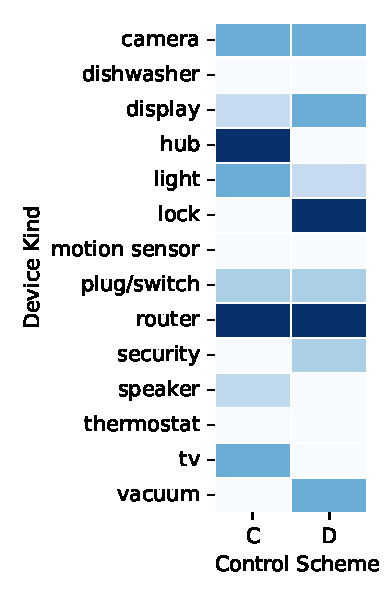
\includegraphics[width=0.333\linewidth]{ControlInContext/figures/control_schemes_vs_dev_kind_pc.pdf}
    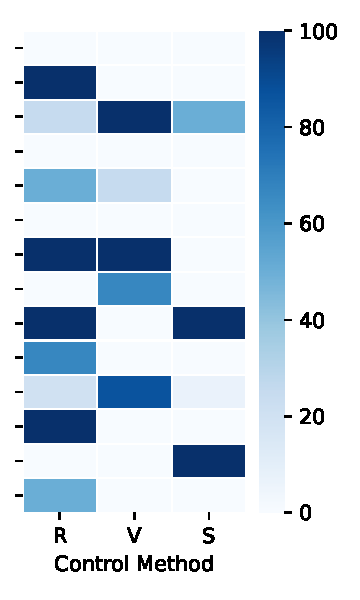
\includegraphics[width=0.313\linewidth]{ControlInContext/figures/control_methods_vs_dev_kind_pc.pdf}
    \caption{Percentage of participants using each control scheme/method vs.\ device kind.
    Participants may refer to a device with a different description from how they most commonly use it, leading to an occasional discrepancy between the device kind and the control method used; for example, a participant may refer to Alexa as only a smart speaker when it is also a hub~\cite{wang2020want,singh2018users, georgiev2018smart}.}
    \medskip
    \label{cic:fig:control-scheme-popularity-vs-dev-kind}
\end{figure}

Survey and interview responses showed that participants rarely commit to a single point on the control spectrum. 
%\del{Instead, they utilized different control methods, such as voice commands, phone applications, routines, and more, depending on the task, device, and context.} 
About half of the survey participants ($51\%$) controlled their devices using voice commands, which can be used across the proxy-based control spectrum. Additionally, $33\%$ of participants reported using routines to control their devices, which allowed them to control groups of devices simultaneously. Furthermore, $18\%$ of participants reported using `content streaming or casting' to control single devices, which is common for media devices such as smart TVs. Both user preferences and device constraints influenced participants' choice of control methods; for instance, participants using Amazon Alexa often relied on voice control due to physical device functionality limitations, while others with broader device ecosystems could select among multiple control methods.

As smart home ecosystems became more complex, participants increasingly shifted toward centralized control by purchasing and using smart home third-party hubs and adopting routines. \Cref{cic:fig:control-scheme-popularity-vs-dev-no} shows that the use of centralized schemes rises alongside the number of devices owned among the survey participants. 

Interview participants who manage many devices reinforced this result, as they reported turning to centralized hubs or voice assistants to reduce the cognitive load of juggling multiple interfaces. 
In particular, interview participant P7, who owned nearly 50 devices, said they relied heavily on central control but acknowledged its limitations: ``\textit{It's not easy to remember [what each device is named].}'' Still, this strategy helped them operate a large-scale setup more efficiently. 

At the same time, users moved along the spectrum toward physical control when centralized systems failed to meet specific needs. This involved falling back to control methods such as physical interaction with a specific device or using a brand-specific application on their phone. Several interview participants noted that detailed settings, such as firmware updates or custom automations, were often only accessible through the device's native app. For example, P3 shared: ``\textit{There is a button in the [Hue] app to make the light bulb that you're trying to interact with, blink on and off, so that you know exactly which one it is; that doesn't exist in the Google app.}'' 

Further, \Cref{cic:fig:control-scheme-popularity-vs-dev-kind} shows that non-central control remains popular for devices requiring more granular or custom interactions, such as security systems or vacuums, where direct control over specific features is necessary. We also observe that participants usually chose to control a device exclusively with either routines or voice commands, but not both.


Some participants used strategies to stay where they were on the control spectrum rather than move along it. Half of the interview participants (4/8), in particular, expressed that they were hesitant to buy new smart home devices that required significant effort to integrate into the existing infrastructure. For example, participants often decided against purchasing devices that required them to download a new application on their phone to set up or use the device. They instead chose to purchase devices that could be controlled using applications already on their phone. P1, when discussing why they purchased a particular brand of new smart device, echoed this sentiment, saying, ``\textit{I already got a lot of apps on my phone. So when possible, I don't wanna put more apps on. So I checked that it'll work with Smart Life. I checked that it's compatible with Alexa.}'' Similarly, P3 described the cost of integrating a new device into their existing smart home control scheme as a significant factor, saying ``\textit{I definitely consider that before buying a potential product, and if possible, I try to buy ones that don't require me to use a new app or ecosystem. There is a cost of switching there that I don't necessarily want to introduce to myself.}'' Participants' responses reflected a desire to gain the benefits (e.g., safety, convenience, etc.) of new smart devices in their home without the potential drawbacks of needing to work outside their home's existing smart device ecosystem, forcing them to adopt mindsets of ``brand loyalty''~\cite{wu2017internet}. 

Long-term use affected user strategies as well. P3 found that as time passed, the scale of the smart home increased, and it \textit{``no longer would be easy to control with just [their] phone,''} enhancing the need for more fine-grained control and more options through more direct control schemes. In contrast, P5 is \textit{``using two providers, Nest and Tapo. I want to choose only from those two the new device,''} and limit the number of interfaces they are using, even if their smart device collection grows. Further, expertise grows over time for some, such as P2: \textit{``for setup, I know now what to do. I've had problems in the past. And I've learned from those problems,''} letting them more comfortably approach new interfaces. Yet, some interfaces are still particularly hard to get used to, as P3 describes having to relearn how to find the routines setup, eroding the trust and patience that users initially have for smart features that centralize control: \textit{``I don't rely on routines for most of the house, except for the room where our animals are.''}
These experiences show how temporal changes in smart home scale or expertise push users to expand or preserve their navigational limits on the control spectrum.

Overall, most participants did not adopt a fixed position on the smart home control spectrum. Instead, they moved fluidly along it, adapting to the demands of scale, task complexity, and reliability using various strategies. In the next section, we examine the specific tradeoffs users perceived and how these influenced their decisions to stay at a certain point or move within the control spectrum.

\subsubsection{Control spectrum navigation tradeoffs (RQ1a)}
\label{cic:subsec:tradeoffs}
While participants demonstrated flexibility in their control strategies, their decisions were shaped by tradeoffs between convenience, precision, cognitive effort, and integration. These tradeoffs were not static; instead, they shifted with the scale of the smart home, the types of devices involved, and the user's comfort with technology. Participants weighed these factors when choosing whether to lean toward centralized control (where a single proxy controls many devices) or physical individual device control at any point in their day.

Participants commonly cited convenience as the most compelling reason for adopting centralized control. This was particularly true as the number of devices in a smart home increased. For example, interview participant P8, who had a large-scale smart home setup, preferred centralized control because it streamlined routine tasks and allowed control through a single interface: ``\textit{It's just obviously the convenience.}'' Survey responses supported this perspective, showing a clear increase in central control-based methods' use among participants with more than 15 devices (\Cref{cic:fig:control-scheme-popularity-vs-dev-no}). Centralized interfaces reduced the friction of opening and switching between multiple apps and offered the possibility of controlling the whole house with fewer steps.
In some cases, these tradeoffs were negotiated within the household rather than by an individual. P6 explained that their partner preferred consolidating under Alexa ``to keep everything easy and streamlined,'' while they themselves ``didn't really care about the brand,'' reflecting how household priorities could drive ecosystem choices.

In contrast, control through second-party interfaces, or per-brand control, was often favored for its granularity, clarity, and ease of use, especially when dealing with specific device configurations or troubleshooting. P2 illustrated this distinction clearly: ``\textit{Whenever I need to adjust something specific, I go straight to the device's own app... Alexa doesn't have those settings.}'' P5 echoed this sentiment, noting that certain features---like firmware updates or custom scenes---were only available in the vendor's own app: ``\textit{Google Home doesn't support [those].}'' This division reveals a tradeoff between breadth and depth: centralized control enabled broad coordination across many devices, but per-brand control offered deeper access to individual brand functionality.

Participants also discussed the usability and user experience differences between central and per-brand control. P3 described centralized interfaces as confusing and overly technical, especially for less tech-savvy users: ``\textit{If you weren't very tech savvy, you would not be able to figure it out.}'' Meanwhile, they described the per-brand app experience as more intuitive and better designed: ``\textit{The Hue app communicates with Hue lights, and that integration is a little bit better.}'' These comparisons underscore how usability and familiarity influenced participants' willingness to rely on one scheme over another.

Not all tradeoffs were framed as strictly negative. Some participants viewed the coexistence of control schemes as beneficial, enabling fallback options or additional layers of control. For instance, participants appreciated having per-brand apps and physical control as a backup when centralized control failed, or vice versa. As P5 described, they would look at a device's specific app first for assistance, rather than the central control system app. Similarly, per-brand apps may also fail and trigger another step down to physical control, as P5 describes: ``\textit{Sometimes it shows as offline because the [brand] app is not able to connect, but the physical device is already up and running. Then I have to turn it off and turn on or do something to get it back up again.''} In these situations, control scheme redundancy offered resilience, not just complexity.

Overall, participants' experiences reveal that smart home control is shaped by ongoing negotiation. Users must continually balance ease of use with technical specificity, minimize app clutter while maximizing access, and integrate new devices without overwhelming themselves. These tradeoffs not only shaped how users controlled devices but also influenced how they structured, grew, and maintained their smart home management systems over time. In the next section, we examine how these navigation strategies and tradeoffs shift when smart home management systems encounter errors and how users respond to breakdowns that disrupt their preferred control methods.


\subsubsection{Navigating the control spectrum when failures occur (RQ2, RQ2a)}
\label{cic:subsec:navigatingcontrol}

While participants developed personalized strategies for navigating the smart home control spectrum, their routines were often disrupted by errors or device failures. These breakdowns forced users to shift control strategies, reconfigure devices, or adopt new troubleshooting behaviors---often in ways that tested the limits of their preferred schemes. Our findings show that errors were a critical moment when users' relationships to the control spectrum changed: participants re-evaluated their trust in control methods, engaged in layered troubleshooting, and sometimes abandoned devices or features altogether.

In the survey, $65\%$ of participants reported that they had experienced at least one issue where a smart device did not work as intended, and $28\%$ reported repeated issues. These issues ranged from connectivity failures ($33\%$), such as devices becoming unresponsive during WiFi outages, to misinterpretation of voice commands ($23\%$) and execution failures, where the device failed to perform the correct task ($21\%$). For instance, one participant noted: ``\textit{When there has been an issue with WiFi in the house, the Amazon Echo tends to have issues.}'' In these moments, control mechanisms that were once trusted became unreliable.

When troubleshooting, participants frequently shifted away from their preferred control methods. For users who primarily relied on central control, their first step was often to check the centralized app or voice assistant interface to confirm whether the command had been sent correctly. Interview participant P7 explained: ``\textit{I will go and look at the app straight away and make sure that the heating has activated rather than just trust it.}'' However, if the centralized interface provided insufficient feedback or failed to offer detailed diagnostics, participants moved toward physical troubleshooting, such as using the vendor app or physically interacting with the device.

Control schemes with very few to no proxies played a crucial role in this context. Many participants described them as more reliable and informative when devices failed. For example, interview participant P5 said they would open the device-specific app to get a clearer view of what had gone wrong. Others, like P8, relied on physical actions like power cycling: ``\textit{And if that doesn't work, I'll just switch it off and back on again.}'' These tactics were rarely described as first-choice methods but were commonly used once central or automated systems proved insufficient.

\begin{figure}[th!]
    \begin{subfigure}{\linewidth}
        \centering
        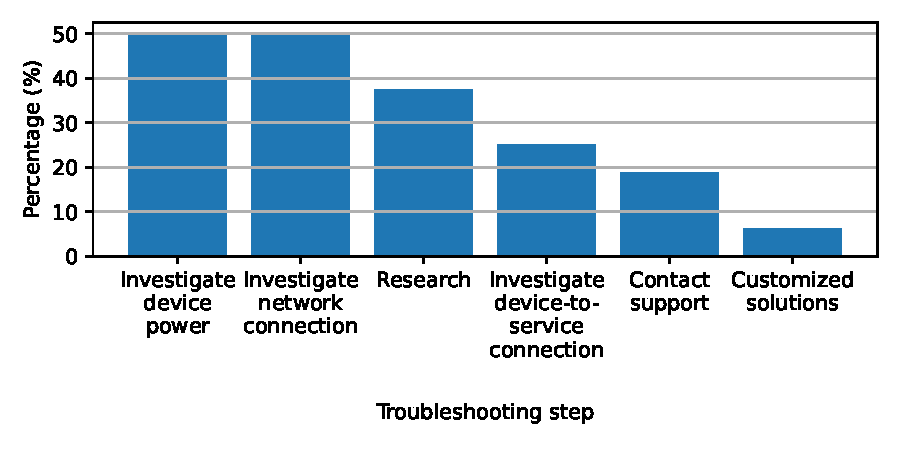
\includegraphics[width=0.7\linewidth]{ControlInContext/figures/survey_troubleshooting_steps_popularity.pdf}
        \caption{Percentage of participants utilizing each troubleshooting step. Each participant may only contribute once towards this metric.}
        % \Description{Bar chart showing the percentage of users performing each troubleshooting step. The most common steps are 'Investigate device power' and 'Investigate network connection', both at 50 percent. These are followed by 'Research' at 38 percent, 'Investigate device-to-service connection' at 25 percent, 'Contact support' at 19 percent, and 'Customized solutions' at 6 percent. The chart illustrates a decreasing trend in user action frequency as steps become more specific or require external assistance.}
        \label{cic:fig:survey-troubleshooting-steps-popularity}
    \end{subfigure}
    \hfill
    \begin{subfigure}{\linewidth}
        \centering
        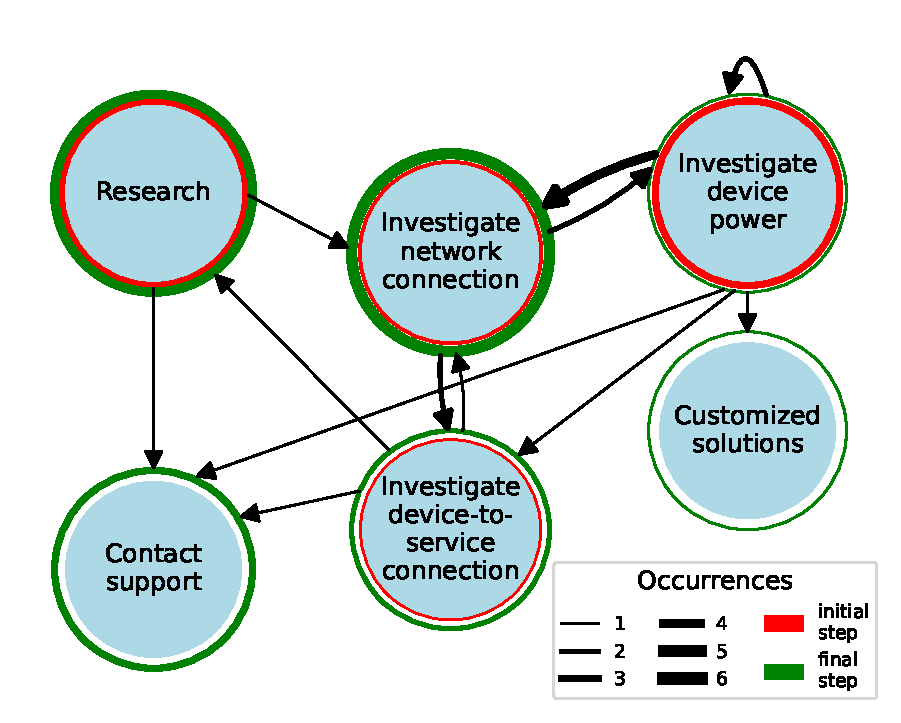
\includegraphics[width=0.6\linewidth]{ControlInContext/figures/survey_troubleshooting_step_sequence.pdf}
        \caption{Troubleshooting step sequence. % %
        A node has a red ring around it if it has been described as an initial step in at least one participant's troubleshooting process. A green ring around a node means it was the final step of one or more participants' troubleshooting process. An arrow links two nodes A, B if at least one participant has gone from step A to step B. The line width of each ring or arrow represents the absolute number of its occurrences across our participants' processes.
        % \todo{write about the skewness of the participant pool who are the main users of the devices}
        }
        % \Description{Flow diagram showing troubleshooting steps and their transition frequencies. Nodes represent steps such as 'Investigate device power', 'Investigate network connection', 'Research', 'Investigate device-to-service connection', 'Contact support', and 'Customized solutions'. Arrows indicate the flow between steps, with line thickness corresponding to frequency of occurrence, ranging from 1 to 6. 'Investigate device power' is the most common initial step, marked with a red inner border, and 'Customized solutions' is the most common final step, marked with a green outer border. Some steps, such as 'Investigate network connection' and 'Investigate device-to-service connection', serve both as intermediates and endpoints. A legend clarifies the line weight and color coding for initial and final steps.}
        \label{cic:fig:survey-troubleshooting-sequence}
    \end{subfigure}
    \caption{Troubleshooting steps results from survey responses. As many are experienced users of their smart home setups, this may subtly shape the emphasis on certain troubleshooting approaches depicted here.
    }
    % \Description{Troubleshooting steps result from survey responses. As many are experienced users of their smart home setups, this may subtly shape the emphasis on certain troubleshooting approaches depicted here.}
    \label{cic:fig:survey-troubleshooting}
\end{figure}

Survey data mirrored these patterns. \Cref{cic:fig:survey-troubleshooting-steps-popularity} shows that $50\%$ of participants restarted the device as part of their troubleshooting process, while $36\%$ restarted or reconnected their device to the internet. Only $12\%$ reported contacting tech support, indicating that most participants tried to resolve issues independently using a set of well-practiced responses. \Cref{cic:fig:survey-troubleshooting-sequence} visualizes the common sequences users followed when troubleshooting. Initial steps often included power or connectivity checks, followed by deeper exploration through brand-specific apps, web research ($22\%$), and more.

Participants also described emotional responses to persistent failures. For some, repeated breakdowns led to troubleshooting fatigue or abandonment. Interview participant P6 shared that a voice-controlled TV consistently misunderstood commands, leading them to eventually ``\textit{give up on it for a long time}'' before replacing the device entirely. While only $9\%$ of survey participants said they returned a device after an error, and $11\%$ said they gave up entirely on a type of device, these moments marked important shifts in how users related to control schemes and whether they were willing to continue adapting.

Notably, participants' troubleshooting practices revealed that they often understood control methods as part of the problem space. For instance, P7 mentioned researching whether thermostat failures were due to device issues or miscommunication with their central control platform. When troubleshooting failed, users sometimes restructured their systems--switching platforms, removing routines, or replacing devices that didn't integrate well with others, as P5 said: ``\textit{[My Kasa switch] was not able to integrate correctly. I had to pair it every time with the Google Home App and every time it would disconnect. And then I had to do it again. And it was painful. So I ended up returning the device.}'' Similarly, P1 described how after an extended period of troubleshooting, they had \textit{``resigned myself to just using the app.''} In these experiences, participants found themselves forced into a particular control method, rather than having autonomy over how they \textit{wanted} to control the device.

Overall, device failures and errors forced participants to switch between control schemes, uncovering limitations and prompting changes to their routine. While many relied on layered troubleshooting strategies, persistent problems sometimes led to long-term shifts in user behavior, feature abandonment, or restructuring of control ecosystems. These findings show that the smart home control spectrum is not only navigated during setup or steady-state use but also actively re-navigated in moments of breakdown.


\subsubsection{Discoverability Failures across the Control Spectrum (RQ2b)}
% \subsection{User Confusion in Locating Smart Home Functionality across the Spectrum}
\label{cic:sec:confusion}

Our interviews reveal that users frequently struggle to realize their intended goals with smart home systems, not because functionality is absent, but because its integration or accessibility---whether in terms of location, when it is available, or how it is surfaced---is unclear.

We identify five recurring categories of confusion and elaborate on each below. \Cref{cic:tab:confusion} summarizes all these categories, including relevant quotes from interviewees.

% \begin{table}[t]
% \centering
% \caption{\add{Taxonomy of user confusion in executing smart home functionality.}}
%    \bigskip
% \label{cic:tab:confusion}
% \color{blue}
% \begin{tabular}{R{4.8cm}|p{10.5cm}}
% \hline
% \textbf{Category} & \textbf{Description and Example Quotes} \\
% \hline\hline
% Fragmented control (central vs. vendor) 
% & Users unsure which app (hub vs. vendor) exposes functionality. 
% \textit{Example:} ``In the Nest app you can see the history... but not on Google Home.'' (N3) \\
% \hline

% \multirow{2}{*}{Hidden / hard-to-find features}
% & Poor discoverability of routines, shortcuts, or advanced options. 
% \textit{Example:} ``Every time I go to set a routine, I have to relearn it.'' (N1) \\
% \hline

% \multirow{2}{*}{Missing or partial integrations}
% & Features expected to exist but absent or incomplete. 
% \textit{Example:} ``I can stream the camera, but I can't move it with voice.'' (N3) \\
% \hline

% Ecosystem lock-in \& workarounds 
% & Vendor ecosystems discourage cross-platform setups; workarounds reduce control. 
% \textit{Example:} ``They assume you're Hue or Ikea exclusively.'' (N5) \\
% \hline

% \multirow{2}{*}{Multi-user household challenges}
% & Routines or settings tied to single accounts, limiting family use. 
% \textit{Example:} ``If I add a routine in the Tapo app, [my wife] can't change it.'' (N3) \\
% \hline
% \end{tabular}
%%% \end{table}

\renewcommand{\arraystretch}{1.2}
\begin{table}[t]
    \centering
    \caption{Taxonomy of user confusion in executing smart home functionality.}
    \bigskip
    \label{cic:tab:confusion}
    \tagpdfsetup{table-tagging=false}
    \footnotesize
    \begin{tabular}{R{3.4cm}|p{5.8cm}|p{6cm}}
        \hline
        \textbf{Category} & \textbf{Description} & \textbf{Example Quote} \\
        \hline\hline
        Fragmented control (central vs. vendor)
        & Users unsure which interface (central vs. vendor) exposes functionality. 
        & \textit{``In the Nest app you can see the history... but not on Google Home.''} (P5) \\
        \hline

        Hidden / hard-to-find features
        & Poor discoverability of routines, shortcuts, or advanced options. 
        & \textit{``Every time I go to set a routine, I have to relearn it.''} (P3) \\
        \hline

        Missing or partial integrations
        & Features expected to exist but absent or incomplete. 
        & \textit{``I can stream the camera, but I can't move it with voice.''} (P5) \\
        \hline

        \raggedleft Ecosystem lock-in \& workarounds
        & \raggedright Vendor ecosystems discourage cross-platform setups; workarounds reduce control. 
        & \textit{``They assume you're Hue or IKEA exclusively.''} (P7) \\
        \hline

        Multi-user household challenges
        & Routines or settings tied to single accounts, limiting family use. 
        & \textit{``If I add a routine in the Tapo app, [my wife] can't change it.''} (P5) \\
        \hline
    \end{tabular}
\end{table}

\noindent\textbf{1) Fragmented control between central and vendor apps.}  
Participants' mental models of control schemes often assumed that central hubs (e.g., Google Home, Alexa) could fully replicate vendor apps. When this expectation was violated, users had to switch between apps, leading to uncertainty about which scheme truly ``owned'' a functionality. E.g., \Cref{cic:tab:confusion}--row 1 shows that Nest and Google Home have different features. 

\noindent\textbf{2) Hidden or hard-to-find features.}  
Even when functionality existed, participants' expectations of where it should reside did not align with the app design. Features like routines or shortcuts were buried in menus, clashing with the mental model that everyday actions should be easily accessible. Users who rarely engaged with a particular scheme were especially likely to misremember or misinterpret where to look, e.g., having to locate a feature all over again every time they need it (\Cref{cic:tab:confusion}--row 2). 

\noindent\textbf{3) Missing or partial integrations.}  
Participants often assumed that devices sharing a hub or assistant would integrate seamlessly. When integrations were absent or partial, like camera actuation features (\Cref{cic:tab:confusion}--row 3), this violated their mental model of the hub as a universal coordinator, eroding confidence in central control. 

\noindent\textbf{4) Ecosystem lock-in and workarounds.}  
Users expected that devices across ecosystems could be mixed and matched. When these expectations failed, e.g., accessing IKEA devices from Hue apps (\Cref{cic:tab:confusion}--row 4), they turned to workarounds such as third-party apps. These choices reflect not just technical limitations but users' mental models of what a ``smart'' home should enable. 

\noindent\textbf{5) Multi-user household challenges.}  
Participants assumed that central routines or device automations would be shareable within a household. When vendor apps restricted access to a single account, this clashed with their model of a shared home environment, driving them to central hubs despite their own limitations. For instance, Tapo does not allow multiple household members (\Cref{cic:tab:confusion}--row 5). 

Across all categories, confusion arose less from the outright absence of functionality than from mismatches between participants' mental models and system design. Users expected hubs to be universal, apps to be intuitive, integrations to be complete, and households to be collaborative. In practice, however, they lacked a clear taxonomy of where functionality resides, how it should be invoked, and whether it integrates with other devices. These findings show that confusion is not just an isolated annoyance but a systemic barrier that reshapes how users perceive and navigate smart home control schemes, influencing when they trust central control, fall back to vendor apps, or abandon features altogether.


